% ----------------------------------------------------------------------
%
%                          Tesis.tex
%
%----------------------------------------------------------------------
%
% Este fichero contiene el "documento maestro" del documento. Lo único
% que hace es configurar el entorno LaTeX e incluir los ficheros .tex
% que contienen cada sección.
%
%----------------------------------------------------------------------
%
% Los ficheros necesarios para este documento son:
%
%       TeXiS/* : ficheros de la plantilla TeXiS.
%       Cascaras/* : ficheros con las partes del documento que no
%          son capítulos ni apéndices (portada, agradecimientos, etc.)
%       Capitulos/*.tex : capítulos de la tesis
%       Apendices/*.tex: apéndices de la tesis
%       constantes.tex: constantes LaTeX
%       config.tex : configuración de la "compilación" del documento
%       guionado.tex : palabras con guiones
%
% Para la bibliografía, además, se necesitan:
%
%       *.bib : ficheros con la información de las referencias
%
% ---------------------------------------------------------------------

\documentclass[12pt,letterpaper,oneside]{book}

%
% Definimos  el   comando  \compilaCapitulo,  que   luego  se  utiliza
% (opcionalmente) en config.tex. Quedaría  mejor si también se definiera
% en  ese fichero,  pero por  el modo  en el  que funciona  eso  no es
% posible. Puedes consultar la documentación de ese fichero para tener
% m�s  información. Definimos también  \compilaApendice, que  tiene el
% mismo  cometido, pero  que se  utiliza para  compilar  únicamente un
% apéndice.
%
%
% Si  queremos   compilar  solo   una  parte  del   documento  podemos
% especificar mediante  \includeonly{...} qué ficheros  son los únicos
% que queremos  que se incluyan.  Esto  es útil por  ejemplo para sólo
% compilar un capítulo.
%
% El problema es que todos aquellos  ficheros que NO est�n en la lista
% NO   se  incluirán...  y   eso  también   afecta  a   ficheros  de
% la plantilla...
%
% Total,  que definimos  una constante  con los  ficheros  que siempre
% vamos a querer compilar  (aquellos relacionados con configuración) y
% luego definimos \compilaCapitulo.
\newcommand{\ficherosBasicosTeXiS}{%
TeXiS/TeXiS_pream,TeXiS/TeXiS_cab,TeXiS/TeXiS_bib,TeXiS/TeXiS_cover,%
TeXiS/TeXiS_part%
}
\newcommand{\ficherosBasicosTexto}{%
constantes,guionado,Cascaras/bibliografia,config%
}
\newcommand{\compilaCapitulo}[1]{%
\includeonly{\ficherosBasicosTeXiS,\ficherosBasicosTexto,Capitulos/#1}%
}

\newcommand{\compilaApendice}[1]{%
\includeonly{\ficherosBasicosTeXiS,\ficherosBasicosTexto,Apendices/#1}%
}

%- - - - - - - - - - - - - - - - - - - - - - - - - - - - - - - - - - -
%            Preámbulo del documento. Configuraciones varias
%- - - - - - - - - - - - - - - - - - - - - - - - - - - - - - - - - - -

% Define  el  tipo  de  compilación que  estamos  haciendo.   Contiene
% definiciones  de  constantes que  cambian  el  comportamiento de  la
% compilación. Debe incluirse antes del paquete TeXiS/TeXiS.sty
%---------------------------------------------------------------------
%
%                          config.tex
%
%---------------------------------------------------------------------
%
% Contiene la  definición de constantes  que determinan el modo  en el
% que se compilar� el documento.
%
%---------------------------------------------------------------------
%
% En concreto, podemos  indicar si queremos "modo release",  en el que
% no  aparecerán  los  comentarios  (creados  mediante  \com{Texto}  o
% \comp{Texto}) ni los "por  hacer" (creados mediante \todo{Texto}), y
% sí aparecerán los índices. El modo "debug" (o mejor dicho en modo no
% "release" muestra los índices  (construirlos lleva tiempo y son poco
% útiles  salvo  para   la  versión  final),  pero  sí   el  resto  de
% anotaciones.
%
% Si se compila con LaTeX (no  con pdflatex) en modo Debug, tambi�n se
% muestran en una esquina de cada página las entradas (en el índice de
% palabras) que referencian  a dicha página (consulta TeXiS_pream.tex,
% en la parte referente a show).
%
% El soporte para  el índice de palabras en  TeXiS es embrionario, por
% lo  que no  asumas que  esto funcionará  correctamente.  Consulta la
% documentación al respecto en TeXiS_pream.tex.
%
%
% También  aquí configuramos  si queremos  o  no que  se incluyan  los
% acrónimos  en el  documento final  en la  versión release.  Para eso
% define (o no) la constante \acronimosEnRelease.
%
% Utilizando \compilaCapitulo{nombre}  podemos también especificar qué
% capítulo(s) queremos que se compilen. Si no se pone nada, se compila
% el documento  completo.  Si se pone, por  ejemplo, 01Introduccion se
% compilará únicamente el fichero Capitulos/01Introduccion.tex
%
% Para compilar varios  capítulos, se separan sus nombres  con comas y
% no se ponen espacios de separación.
%
% En realidad  la macro \compilaCapitulo  está definida en  el fichero
% principal tesis.tex.
%
%---------------------------------------------------------------------


% Comentar la l�nea si no se compila en modo release.
% TeXiS hará el resto.
% ¡¡¡Si cambias esto, haz un make clean antes de recompilar!!!
\def\release{1}


% Descomentar la linea si se quieren incluir los
% acrónimos en modo release (en modo debug
% no se incluirán nunca).
% ¡¡¡Si cambias esto, haz un make clean antes de recompilar!!!
\def\acronimosEnRelease{1}


% Descomentar la línea para establecer el capítulo que queremos
% compilar

% \compilaCapitulo{01Introduccion}
% \compilaCapitulo{02EstructuraYGeneracion}
% \compilaCapitulo{03Edicion}
% \compilaCapitulo{04Imagenes}
% \compilaCapitulo{05Bibliografia}
% \compilaCapitulo{06Makefile}

% \compilaApendice{01AsiSeHizo}

% Variable local para emacs, para  que encuentre el fichero maestro de
% compilación y funcionen mejor algunas teclas rápidas de AucTeX
%%%
%%% Local Variables:
%%% mode: latex
%%% TeX-master: "./Tesis.tex"
%%% End:


% Paquete de la plantilla
\usepackage{TeXiS/TeXiS}

% Incluimos el fichero con comandos de constantes
%---------------------------------------------------------------------
%
%                          constantes.tex
%
%---------------------------------------------------------------------
%
% Fichero que  declara nuevos comandos LaTeX  sencillos realizados por
% comodidad en la escritura de determinadas palabras
%
%---------------------------------------------------------------------

%%%%%%%%%%%%%%%%%%%%%%%%%%%%%%%%%%%%%%%%%%%%%%%%%%%%%%%%%%%%%%%%%%%%%%
% Comando: 
%
%       \titulo
%
% Resultado: 
%
% Escribe el título del documento.
%%%%%%%%%%%%%%%%%%%%%%%%%%%%%%%%%%%%%%%%%%%%%%%%%%%%%%%%%%%%%%%%%%%%%%
\def\titulo{\textsc{TeXiS}: Una plantilla de \LaTeX\
  para Tesis y otros documentos}

%%%%%%%%%%%%%%%%%%%%%%%%%%%%%%%%%%%%%%%%%%%%%%%%%%%%%%%%%%%%%%%%%%%%%%
% Comando: 
%
%       \autor
%
% Resultado: 
%
% Escribe el autor del documento.
%%%%%%%%%%%%%%%%%%%%%%%%%%%%%%%%%%%%%%%%%%%%%%%%%%%%%%%%%%%%%%%%%%%%%%
\def\autor{Marco Antonio y Pedro Pablo G\'omez Mart\'in}

% Variable local para emacs, para  que encuentre el fichero maestro de
% compilaci�n y funcionen mejor algunas teclas r�pidas de AucTeX

%%%
%%% Local Variables:
%%% mode: latex
%%% TeX-master: "tesis.tex"
%%% End:


% Sacamos en el log de la compilación el copyright
\typeout{Copyright Marco Antonio and Pedro Pablo Gomez Martin}

%
% "Metadatos" para el PDF
%
\ifpdf\hypersetup{%
    pdftitle = {\titulo},
    pdfsubject = {Plantilla de Tesis},
    pdfkeywords = {Plantilla, LaTeX, tesis, trabajo de
      investigación, trabajo de Master},
    pdfauthor = {\textcopyright\ \autor},
    pdfcreator = {\LaTeX\ con el paquete \flqq hyperref\frqq},
    pdfproducer = {pdfeTeX-0.\the\pdftexversion\pdftexrevision},
    }
    \pdfinfo{/CreationDate (\today)}
\fi


%- - - - - - - - - - - - - - - - - - - - - - - - - - - - - - - - - - -
%                        Documento
%- - - - - - - - - - - - - - - - - - - - - - - - - - - - - - - - - - -
% Asignamos margen de 1 pulgada (1in)
\geometry{margin=1in}

\begin{document}

% Incluimos el  fichero de definición de guionado  de algunas palabras
% que LaTeX no ha dividido como debería
%----------------------------------------------------------------
%
%                          guionado.tex
%
%----------------------------------------------------------------
%
% Fichero con algunas divisiones de palabras que LaTeX no
% hace correctamente si no se le da alguna ayuda.
%
%----------------------------------------------------------------

\hyphenation{
% a
abs-trac-to
abs-trac-tos
abs-trac-ta
abs-trac-tas
ac-tua-do-res
a-gra-de-ci-mien-tos
ana-li-za-dor
an-te-rio-res
an-te-rior-men-te
apa-rien-cia
a-pro-pia-do
a-pro-pia-dos
a-pro-pia-da
a-pro-pia-das
a-pro-ve-cha-mien-to
a-que-llo
a-que-llos
a-que-lla
a-que-llas
a-sig-na-tu-ra
a-sig-na-tu-ras
a-so-cia-da
a-so-cia-das
a-so-cia-do
a-so-cia-dos
au-to-ma-ti-za-do
% b
batch
bi-blio-gra-f�a
bi-blio-gr�-fi-cas
bien
bo-rra-dor
boo-l-ean-expr
% c
ca-be-ce-ra
call-me-thod-ins-truc-tion
cas-te-lla-no
cir-cuns-tan-cia
cir-cuns-tan-cias
co-he-ren-te
co-he-ren-tes
co-he-ren-cia
co-li-bri
co-men-ta-rio
co-mer-cia-les
co-no-ci-mien-to
cons-cien-te
con-si-de-ra-ba
con-si-de-ra-mos
con-si-de-rar-se
cons-tan-te
cons-trucci�n
cons-tru-ye
cons-tru-ir-se
con-tro-le
co-rrec-ta-men-te
co-rres-pon-den
co-rres-pon-dien-te
co-rres-pon-dien-tes
co-ti-dia-na
co-ti-dia-no
crean
cris-ta-li-zan
cu-rri-cu-la
cu-rri-cu-lum
cu-rri-cu-lar
cu-rri-cu-la-res
% d
de-di-ca-do
de-di-ca-dos
de-di-ca-da
de-di-ca-das
de-rro-te-ro
de-rro-te-ros
de-sa-rro-llo
de-sa-rro-llos
de-sa-rro-lla-do
de-sa-rro-lla-dos
de-sa-rro-lla-da
de-sa-rro-lla-das
de-sa-rro-lla-dor
de-sa-rro-llar
des-cri-bi-re-mos
des-crip-ci�n
des-crip-cio-nes
des-cri-to
des-pu�s
de-ta-lla-do
de-ta-lla-dos
de-ta-lla-da
de-ta-lla-das
di-a-gra-ma
di-a-gra-mas
di-se-�os
dis-po-ner
dis-po-ni-bi-li-dad
do-cu-men-ta-da
do-cu-men-to
do-cu-men-tos
% e
edi-ta-do
e-du-ca-ti-vo
e-du-ca-ti-vos
e-du-ca-ti-va
e-du-ca-ti-vas
e-la-bo-ra-do
e-la-bo-ra-dos
e-la-bo-ra-da
e-la-bo-ra-das
es-co-llo
es-co-llos
es-tu-dia-do
es-tu-dia-dos
es-tu-dia-da
es-tu-dia-das
es-tu-dian-te
e-va-lua-cio-nes
e-va-lua-do-res
exis-ten-tes
exhaus-ti-va
ex-pe-rien-cia
ex-pe-rien-cias
% f
for-ma-li-za-do
% g
ge-ne-ra-ci�n
ge-ne-ra-dor
ge-ne-ra-do-res
ge-ne-ran
% h
he-rra-mien-ta
he-rra-mien-tas
% i
i-dio-ma
i-dio-mas
im-pres-cin-di-ble
im-pres-cin-di-bles
in-de-xa-do
in-de-xa-dos
in-de-xa-da
in-de-xa-das
in-di-vi-dual
in-fe-ren-cia
in-fe-ren-cias
in-for-ma-ti-ca
in-gre-dien-te
in-gre-dien-tes
in-me-dia-ta-men-te
ins-ta-la-do
ins-tan-cias
% j
% k
% l
len-gua-je
li-be-ra-to-rio
li-be-ra-to-rios
li-be-ra-to-ria
li-be-ra-to-rias
li-mi-ta-do
li-te-ra-rio
li-te-ra-rios
li-te-ra-ria
li-te-ra-rias
lo-tes
% m
ma-ne-ra
ma-nual
mas-que-ra-de
ma-yor
me-mo-ria
mi-nis-te-rio
mi-nis-te-rios
mo-de-lo
mo-de-los
mo-de-la-do
mo-du-la-ri-dad
mo-vi-mien-to
% n
na-tu-ral
ni-vel
nues-tro
% o
obs-tan-te
o-rien-ta-do
o-rien-ta-dos
o-rien-ta-da
o-rien-ta-das
% p
pa-ra-le-lo
pa-ra-le-la
par-ti-cu-lar
par-ti-cu-lar-men-te
pe-da-g�-gi-ca
pe-da-g�-gi-cas
pe-da-g�-gi-co
pe-da-g�-gi-cos
pe-rio-di-ci-dad
per-so-na-je
plan-te-a-mien-to
plan-te-a-mien-tos
po-si-ci�n
pre-fe-ren-cia
pre-fe-ren-cias
pres-cin-di-ble
pres-cin-di-bles
pri-me-ra
pro-ble-ma
pro-ble-mas
pr�-xi-mo
pu-bli-ca-cio-nes
pu-bli-ca-do
% q
% r
r�-pi-da
r�-pi-do
ra-zo-na-mien-to
ra-zo-na-mien-tos
re-a-li-zan-do
re-fe-ren-cia
re-fe-ren-cias
re-fe-ren-cia-da
re-fe-ren-cian
re-le-van-tes
re-pre-sen-ta-do
re-pre-sen-ta-dos
re-pre-sen-ta-da
re-pre-sen-ta-das
re-pre-sen-tar-lo
re-qui-si-to
re-qui-si-tos
res-pon-der
res-pon-sa-ble
% s
se-pa-ra-do
si-guien-do
si-guien-te
si-guien-tes
si-guie-ron
si-mi-lar
si-mi-la-res
si-tua-ci�n
% t
tem-pe-ra-ments
te-ner
trans-fe-ren-cia
trans-fe-ren-cias
% u
u-sua-rio
Unreal-Ed
% v
va-lor
va-lo-res
va-rian-te
ver-da-de-ro
ver-da-de-ros
ver-da-de-ra
ver-da-de-ras
ver-da-de-ra-men-te
ve-ri-fi-ca
% w
% x
% y
% z
}
% Variable local para emacs, para que encuentre el fichero
% maestro de compilaci�n
%%%
%%% Local Variables:
%%% mode: latex
%%% TeX-master: "./Tesis.tex"
%%% End:


% Marcamos  el inicio  del  documento para  la  numeración de  páginas
% (usando números romanos para esta primera fase).
\frontmatter

%---------------------------------------------------------------------
%
%                          configCover.tex
%
%---------------------------------------------------------------------
%
% cover.tex
% Copyright 2009 Marco Antonio Gomez-Martin, Pedro Pablo Gomez-Martin
%
% This file belongs to the TeXiS manual, a LaTeX template for writting
% Thesis and other documents. The complete last TeXiS package can
% be obtained from http://gaia.fdi.ucm.es/projects/texis/
%
% Although the TeXiS template itself is distributed under the 
% conditions of the LaTeX Project Public License
% (http://www.latex-project.org/lppl.txt), the manual content
% uses the CC-BY-SA license that stays that you are free:
%
%    - to share & to copy, distribute and transmit the work
%    - to remix and to adapt the work
%
% under the following conditions:
%
%    - Attribution: you must attribute the work in the manner
%      specified by the author or licensor (but not in any way that
%      suggests that they endorse you or your use of the work).
%    - Share Alike: if you alter, transform, or build upon this
%      work, you may distribute the resulting work only under the
%      same, similar or a compatible license.
%
% The complete license is available in
% http://creativecommons.org/licenses/by-sa/3.0/legalcode
%
%---------------------------------------------------------------------
%
% Fichero que contiene la configuraci�n de la portada y de la 
% primera hoja del documento.
%
%---------------------------------------------------------------------


% Pueden configurarse todos los elementos del contenido de la portada
% utilizando comandos.

%%%%%%%%%%%%%%%%%%%%%%%%%%%%%%%%%%%%%%%%%%%%%%%%%%%%%%%%%%%%%%%%%%%%%%
% Instituci�n/departamento asociado al documento.
% \institucion{Nombre}
% Puede tener varias l�neas. Se utiliza en las dos portadas.
% Si no se indica aparecer� vac�o.
%%%%%%%%%%%%%%%%%%%%%%%%%%%%%%%%%%%%%%%%%%%%%%%%%%%%%%%%%%%%%%%%%%%%%%
\institucion{%
UNIVERSIDAD AUT\'ONOMA "GABRIEL REN\'E MORENO"\\ [0.2em]
FACULTAD DE INGENIER\'IA EN CIENCIAS DE LA COMPUTACI\'ON Y TELECOMUNICACIONES\\ [0.2em]
"UAGRM SCHOOL OF ENGINEERING"
}

%%%%%%%%%%%%%%%%%%%%%%%%%%%%%%%%%%%%%%%%%%%%%%%%%%%%%%%%%%%%%%%%%%%%%%
% T�tulo del documento:
% \tituloPortada{titulo}
% Nota:
% Si no se define se utiliza el del \titulo. Este comando permite
% cambiar el t�tulo de forma que se especifiquen d�nde se quieren
% los retornos de carro cuando se utilizan fuentes grandes.
%%%%%%%%%%%%%%%%%%%%%%%%%%%%%%%%%%%%%%%%%%%%%%%%%%%%%%%%%%%%%%%%%%%%%%
\tituloPortada{%
\texis: Una plantilla de \LaTeX\\
para Tesis y otros documentos%
}

%%%%%%%%%%%%%%%%%%%%%%%%%%%%%%%%%%%%%%%%%%%%%%%%%%%%%%%%%%%%%%%%%%%%%%
% Autor del documento:
% \autorPortada{Nombre}
% Se utiliza en la portada y en el valor por defecto del
% primer subt�tulo de la segunda portada.
%%%%%%%%%%%%%%%%%%%%%%%%%%%%%%%%%%%%%%%%%%%%%%%%%%%%%%%%%%%%%%%%%%%%%%
\autorPortada{Marco Antonio G�mez Mart�n\\Pedro Pablo G�mez Mart�n}

%%%%%%%%%%%%%%%%%%%%%%%%%%%%%%%%%%%%%%%%%%%%%%%%%%%%%%%%%%%%%%%%%%%%%%
% Fecha de publicaci�n:
% \fechaPublicacion{Fecha}
% Puede ser vac�o. Aparece en la �ltima l�nea de ambas portadas
%%%%%%%%%%%%%%%%%%%%%%%%%%%%%%%%%%%%%%%%%%%%%%%%%%%%%%%%%%%%%%%%%%%%%%
\fechaPublicacion{Noviembre 2009}

%%%%%%%%%%%%%%%%%%%%%%%%%%%%%%%%%%%%%%%%%%%%%%%%%%%%%%%%%%%%%%%%%%%%%%
% Imagen de la portada (y escala)
% \imagenPortada{Fichero}
% \escalaImagenPortada{Numero}
% Si no se especifica, se utiliza la imagen TODO.pdf
%%%%%%%%%%%%%%%%%%%%%%%%%%%%%%%%%%%%%%%%%%%%%%%%%%%%%%%%%%%%%%%%%%%%%%
\imagenPortada{Imagenes/Vectorial/UAGRMEscudoSOE}
\escalaImagenPortada{1.0}

%%%%%%%%%%%%%%%%%%%%%%%%%%%%%%%%%%%%%%%%%%%%%%%%%%%%%%%%%%%%%%%%%%%%%%
% Tipo de documento.
% \tipoDocumento{Tipo}
% Para el texto justo debajo del escudo.
% Si no se indica, se utiliza "TESIS DOCTORAL".
%%%%%%%%%%%%%%%%%%%%%%%%%%%%%%%%%%%%%%%%%%%%%%%%%%%%%%%%%%%%%%%%%%%%%%
\tipoDocumento{MANUAL DE USUARIO}

%%%%%%%%%%%%%%%%%%%%%%%%%%%%%%%%%%%%%%%%%%%%%%%%%%%%%%%%%%%%%%%%%%%%%%
% Director del trabajo.
% \directorPortada{Nombre}
% Se utiliza para el valor por defecto del segundo subt�tulo, donde
% se indica qui�n es el director del trabajo.
% Si se fuerza un subt�tulo distinto, no hace falta definirlo.
%%%%%%%%%%%%%%%%%%%%%%%%%%%%%%%%%%%%%%%%%%%%%%%%%%%%%%%%%%%%%%%%%%%%%%
%\directorPortada{Walterio Malatesta}

%%%%%%%%%%%%%%%%%%%%%%%%%%%%%%%%%%%%%%%%%%%%%%%%%%%%%%%%%%%%%%%%%%%%%%
% Texto del primer subt�tulo de la segunda portada.
% \textoPrimerSubtituloPortada{Texto}
% Para configurar el primer "texto libre" de la segunda portada.
% Si no se especifica se indica "Memoria que presenta para optar al
% t�tulo de Doctor en Inform�tica" seguido del \autorPortada.
%%%%%%%%%%%%%%%%%%%%%%%%%%%%%%%%%%%%%%%%%%%%%%%%%%%%%%%%%%%%%%%%%%%%%%
\textoPrimerSubtituloPortada{%
\textit{Informe t�cnico del departamento}  \\ [0.3em]
\textbf{Ingenier�a del Software e Inteligencia Artificial} \\ [0.3em]
\textbf{IT/2009/3}
}

%%%%%%%%%%%%%%%%%%%%%%%%%%%%%%%%%%%%%%%%%%%%%%%%%%%%%%%%%%%%%%%%%%%%%%
% Texto del segundo subt�tulo de la segunda portada.
% \textoSegundoSubtituloPortada{Texto}
% Para configurar el segundo "texto libre" de la segunda portada.
% Si no se especifica se indica "Dirigida por el Doctor" seguido
% del \directorPortada.
%%%%%%%%%%%%%%%%%%%%%%%%%%%%%%%%%%%%%%%%%%%%%%%%%%%%%%%%%%%%%%%%%%%%%%
\textoSegundoSubtituloPortada{%
\textit{Versi�n \texisVer}
}

%%%%%%%%%%%%%%%%%%%%%%%%%%%%%%%%%%%%%%%%%%%%%%%%%%%%%%%%%%%%%%%%%%%%%%
% \explicacionDobleCara
% Si se utiliza, se aclara que el documento est� preparado para la
% impresi�n a doble cara.
%%%%%%%%%%%%%%%%%%%%%%%%%%%%%%%%%%%%%%%%%%%%%%%%%%%%%%%%%%%%%%%%%%%%%%
\explicacionDobleCara

%%%%%%%%%%%%%%%%%%%%%%%%%%%%%%%%%%%%%%%%%%%%%%%%%%%%%%%%%%%%%%%%%%%%%%
% \isbn
% Si se utiliza, aparecer� el ISBN detr�s de la segunda portada.
%%%%%%%%%%%%%%%%%%%%%%%%%%%%%%%%%%%%%%%%%%%%%%%%%%%%%%%%%%%%%%%%%%%%%%
\isbn{978-84-692-7109-4}


%%%%%%%%%%%%%%%%%%%%%%%%%%%%%%%%%%%%%%%%%%%%%%%%%%%%%%%%%%%%%%%%%%%%%%
% \copyrightInfo
% Si se utiliza, aparecer� informaci�n de los derechos de copyright
% detr�s de la segunda portada.
%%%%%%%%%%%%%%%%%%%%%%%%%%%%%%%%%%%%%%%%%%%%%%%%%%%%%%%%%%%%%%%%%%%%%%
\copyrightInfo{\autor}


%%
%% Creamos las portadas
%%
\makeCover

% Variable local para emacs, para que encuentre el fichero
% maestro de compilaci�n
%%%
%%% Local Variables:
%%% mode: latex
%%% TeX-master: "../Tesis.tex"
%%% End:


%---------------------------------------------------------------------
%
%                      dedicatoria.tex
%
%---------------------------------------------------------------------
%
% dedicatoria.tex
% Copyright 2009 Marco Antonio Gomez-Martin, Pedro Pablo Gomez-Martin
%
% This file belongs to the TeXiS manual, a LaTeX template for writting
% Thesis and other documents. The complete last TeXiS package can
% be obtained from http://gaia.fdi.ucm.es/projects/texis/
%
% Although the TeXiS template itself is distributed under the 
% conditions of the LaTeX Project Public License
% (http://www.latex-project.org/lppl.txt), the manual content
% uses the CC-BY-SA license that stays that you are free:
%
%    - to share & to copy, distribute and transmit the work
%    - to remix and to adapt the work
%
% under the following conditions:
%
%    - Attribution: you must attribute the work in the manner
%      specified by the author or licensor (but not in any way that
%      suggests that they endorse you or your use of the work).
%    - Share Alike: if you alter, transform, or build upon this
%      work, you may distribute the resulting work only under the
%      same, similar or a compatible license.
%
% The complete license is available in
% http://creativecommons.org/licenses/by-sa/3.0/legalcode
%
%---------------------------------------------------------------------
%
% Contiene la p�gina de dedicatorias.
%
%---------------------------------------------------------------------

\dedicatoriaUno{%
\emph{
Al duque de B�jar\\
y\hspace*{10ex} \\
a t�, lector car�simo%
}%
}

\dedicatoriaDos{%
\emph{%
I can't go to a restaurant and\\%
order food because I keep looking\\%
at the fonts on the menu.\\%
Donald Knuth%
}%
}

\makeDedicatorias

% Variable local para emacs, para que encuentre el fichero
% maestro de compilaci�n
%%%
%%% Local Variables:
%%% mode: latex
%%% TeX-master: "../Tesis.tex"
%%% End:


%---------------------------------------------------------------------
%
%                      agradecimientos.tex
%
%---------------------------------------------------------------------
%
% agradecimientos.tex
% Copyright 2009 Marco Antonio Gomez-Martin, Pedro Pablo Gomez-Martin
%
% This file belongs to the TeXiS manual, a LaTeX template for writting
% Thesis and other documents. The complete last TeXiS package can
% be obtained from http://gaia.fdi.ucm.es/projects/texis/
%
% Although the TeXiS template itself is distributed under the 
% conditions of the LaTeX Project Public License
% (http://www.latex-project.org/lppl.txt), the manual content
% uses the CC-BY-SA license that stays that you are free:
%
%    - to share & to copy, distribute and transmit the work
%    - to remix and to adapt the work
%
% under the following conditions:
%
%    - Attribution: you must attribute the work in the manner
%      specified by the author or licensor (but not in any way that
%      suggests that they endorse you or your use of the work).
%    - Share Alike: if you alter, transform, or build upon this
%      work, you may distribute the resulting work only under the
%      same, similar or a compatible license.
%
% The complete license is available in
% http://creativecommons.org/licenses/by-sa/3.0/legalcode
%
%---------------------------------------------------------------------
%
% Contiene la p�gina de agradecimientos.
%
% Se crea como un cap�tulo sin numeraci�n.
%
%---------------------------------------------------------------------

\chapter{Agradecimientos}

\cabeceraEspecial{Agradecimientos}

\begin{FraseCelebre}
\begin{Frase}
A todos los que la presente vieren y entendieren.
\end{Frase}
\begin{Fuente}
Inicio de las Leyes Org�nicas. Juan Carlos I
\end{Fuente}
\end{FraseCelebre}

Groucho Marx dec�a que encontraba a la televisi�n muy educativa porque
cada vez que alguien la encend�a, �l se iba a otra habitaci�n a leer
un libro. Utilizando un esquema similar, nosotros queremos agradecer
al Word de Microsoft el habernos forzado a utilizar \LaTeX. Cualquiera
que haya intentado escribir un documento de m�s de 150 p�ginas con
esta aplicaci�n entender� a qu� nos referimos. Y lo decimos porque
nuestra andadura con \LaTeX\ comenz�, precisamente, despu�s de
escribir un documento de algo m�s de 200 p�ginas. Una vez terminado
decidimos que nunca m�s pasar�amos por ah�. Y entonces ca�mos en
\LaTeX.

Es muy posible que hub�eramos llegado al mismo sitio de todas formas,
ya que en el mundo acad�mico a la hora de escribir art�culos y
contribuciones a congresos lo m�s extendido es \LaTeX. Sin embargo,
tambi�n es cierto que cuando intentas escribir un documento grande
en \LaTeX\ por tu cuenta y riesgo sin un enlace del tipo ``\emph{Author
  instructions}'', se hace cuesta arriba, pues uno no sabe por donde
empezar.

Y ah� es donde debemos agradecer tanto a Pablo Gerv�s como a Miguel
Palomino su ayuda. El primero nos ofreci� el c�digo fuente de una
programaci�n docente que hab�a hecho unos a�os atr�s y que nos sirvi�
de inspiraci�n (por ejemplo, el fichero \texttt{guionado.tex} de
\texis\ tiene una estructura casi exacta a la suya e incluso puede
que el nombre sea el mismo). El segundo nos dej� husmear en el c�digo
fuente de su propia tesis donde, adem�s de otras cosas m�s
interesantes pero menos curiosas, descubrimos que a�n hay gente que
escribe los acentos espa�oles con el \verb+\'{\i}+.

No podemos tampoco olvidar a los numerosos autores de los libros y
tutoriales de \LaTeX\ que no s�lo permiten descargar esos manuales sin
coste adicional, sino que tambi�n dejan disponible el c�digo fuente.
Estamos pensando en Tobias Oetiker, Hubert Partl, Irene Hyna y
Elisabeth Schlegl, autores del famoso ``The Not So Short Introduction
to \LaTeXe'' y en Tom�s Bautista, autor de la traducci�n al espa�ol. De
ellos es, entre otras muchas cosas, el entorno \texttt{example}
utilizado en algunos momentos en este manual.

Tambi�n estamos en deuda con Joaqu�n Ataz L�pez, autor del libro
``Creaci�n de ficheros \LaTeX\ con {GNU} Emacs''. Gracias a �l dejamos
de lado a WinEdt y a Kile, los editores que por entonces utiliz�bamos
en entornos Windows y Linux respectivamente, y nos pasamos a emacs. El
tiempo de escritura que nos ahorramos por no mover las manos del
teclado para desplazar el cursor o por no tener que escribir
\verb+\emph+ una y otra vez se lo debemos a �l; nuestro ocio y vida
social se lo agradecen.

Por �ltimo, gracias a toda esa gente creadora de manuales, tutoriales,
documentaci�n de paquetes o respuestas en foros que hemos utilizado y
seguiremos utilizando en nuestro quehacer como usuarios de
\LaTeX. Sab�is un mont�n.

Y para terminar, a Donal Knuth, Leslie Lamport y todos los que hacen y
han hecho posible que hoy puedas estar leyendo estas l�neas.

\endinput
% Variable local para emacs, para  que encuentre el fichero maestro de
% compilaci�n y funcionen mejor algunas teclas r�pidas de AucTeX
%%%
%%% Local Variables:
%%% mode: latex
%%% TeX-master: "../Tesis.tex"
%%% End:


%---------------------------------------------------------------------
%
%                      resumen.tex
%
%---------------------------------------------------------------------
%
% Contiene el cap�tulo del resumen.
%
% Se crea como un cap�tulo sin numeraci�n.
%
%---------------------------------------------------------------------

\chapter{Resumen}
\cabeceraEspecial{Resumen}

\begin{FraseCelebre}
\begin{Frase}
...
\end{Frase}
\begin{Fuente}
...
\end{Fuente}
\end{FraseCelebre}

...

\endinput
% Variable local para emacs, para  que encuentre el fichero maestro de
% compilaci�n y funcionen mejor algunas teclas r�pidas de AucTeX
%%%
%%% Local Variables:
%%% mode: latex
%%% TeX-master: "../Tesis.tex"
%%% End:


\ifx\generatoc\undefined
\else
%---------------------------------------------------------------------
%
%                          TeXiS_toc.tex
%
%---------------------------------------------------------------------
%
% TeXiS_toc.tex
% Copyright 2009 Marco Antonio Gomez-Martin, Pedro Pablo Gomez-Martin
%
% This file belongs to TeXiS, a LaTeX template for writting
% Thesis and other documents. The complete last TeXiS package can
% be obtained from http://gaia.fdi.ucm.es/projects/texis/
%
% This work may be distributed and/or modified under the
% conditions of the LaTeX Project Public License, either version 1.3
% of this license or (at your option) any later version.
% The latest version of this license is in
%   http://www.latex-project.org/lppl.txt
% and version 1.3 or later is part of all distributions of LaTeX
% version 2005/12/01 or later.
%
% This work has the LPPL maintenance status `maintained'.
% 
% The Current Maintainers of this work are Marco Antonio Gomez-Martin
% and Pedro Pablo Gomez-Martin
%
%---------------------------------------------------------------------
%
% Contiene  los  comandos  para  generar los  índices  del  documento,
% entendiendo por índices las tablas de contenidos.
%
% Genera  el  índice normal  ("tabla  de  contenidos"),  el índice  de
% figuras y el de tablas. También  crea "marcadores" en el caso de que
% se está compilando con pdflatex para que aparezcan en el PDF.
%
%---------------------------------------------------------------------

% FORMATOS DE TÍTULOS
% Capítulo
\titleformat{\chapter}
{\normalfont\large\filcenter\bfseries}{\MakeUppercase{\chaptertitlename}\ \thechapter}{1em}{}

% Seccion
\titleformat{\section}
{\normalfont\normalsize\bfseries}{\thesection}{1em}{}

% Subsección
\titleformat{\subsection}
{\normalfont\normalsize\bfseries}{\thesubsection}{1em}{}

% Agrega un punto (.) al final de las numeraciones
\renewcommand{\thechapter}{\arabic{chapter}.}
\renewcommand{\thesection}{\thechapter\arabic{section}.}
\renewcommand{\thesubsection}{\thesection\arabic{subsection}.}

% Formato del Título de los Índices de Cuadros, Figuras, Anexos
\newcommand{\formattitlelistof}[1]{%
	\thispagestyle{plain}{%
		\begin{center}\textbf{\large #1}\end{center}
	}
}

% Un poquito de configuración...


% Pedimos  que inserte  todos los epígrafes hasta el nivel \subsection
% en la tabla de contenidos.
\setcounter{tocdepth}{2} 

% Le  pedimos  que nos  numere  todos  los  epígrafes hasta  el  nivel
% \subsubsection en el cuerpo del documento.
\setcounter{secnumdepth}{3} 


% Nuevos tipos de listas

% Por defecto LaTeX tiene:
%    - Tabla de contenidos
%    - Índice de figuras
%    - Índice de tablas
% Lo que hace  que  si  necesitamos otros tipos de lista de cosas, por
% ejemplo:  Índice de cuadros,  Índice de ilustraciones, etc.  se debe
% definir, para eso de usa el paquete "tocloft", como dice en:
% https://texblog.org/2008/07/13/define-your-own-list-of/
%
% Ejemplo para listas de elementos de texto:
%    \newcommand{\listXname}{List of Xs}
%    \newlistof{X}{ex}{\listXname}
%    \newcommand{\X}[1]{%
%    \refstepcounter{X}
%    \par\noindent\textbf{X \theexample. #1}
%    \addcontentsline{exp}{example}
%    {\protect\numberline{\thechapter.\theexample}#1}\par}
%
% Ejemplo para listas de elementos flotantes (un elemento flotante por
% defecto son las tablas y las figuras)
%    \newfloat{project}{tbph}{lop}
%    \newcommand{\listprojectname}{List of projects}
%    \newcommand{\listofprojects}{\listof{project}{\thispagestyle{empty} \textbf{\huge \listprojectname}}}


% Índice de cuadros (List of charts)
\newfloat{chart}{tbph}{loch}[chapter]
\floatname{chart}{Cuadro}
\newcommand{\listchartname}{List of charts}
\newcommand{\listofcharts}{\listof{chart}{\formattitlelistof{\listchartname}}}

%
%
% Índice de ilustraciones (List of illustrations)
\newfloat{illustration}{tbph}{loil}[chapter]
\floatname{illustration}{Ilustraci\'on}
\newcommand{\listillustrationname}{List of illustrations}
\newcommand{\listofillustrations}{\listof{illustration}{\formattitlelistof{\listillustrationname}}}

%
%
% Índice de anexos (List of annexes)
\newcommand{\listannexename}{List of charts}
\newcommand{\listofannexes}{\formattitlelistof{\listannexename}}

\newlistof{annexe}{loan}{\listofannexes}
\newcommand{\annexe}[1]{%
\refstepcounter{annexe}
\par\noindent\textbf{Annexe \theannexe. #1}
\addcontentsline{loan}{annexe}
{\protect\numberline{\theannexe}#1}\par}

% Hacemos que las numeraciones de los elementos sean consecutivas
\counterwithout{chart}{chapter}
\counterwithout{table}{chapter}
\counterwithout{figure}{chapter}
\counterwithout{illustration}{chapter}
\counterwithout{annexe}{chapter}


% Creamos los diferentes índices.

% Lo primero un  poco de trabajo en los marcadores  del PDF. No quiero
% que  salga una  entrada  por cada  índice  a nivel  0...  si no  que
% aparezca un marcador "índices", que  tenga dentro los otros tipos de
% índices.  Total, que creamos el marcador "índices".
% Antes de  la creación  de los índices,  se añaden los  marcadores de
% nivel 1.

\ifpdf
   \pdfbookmark{\'Indices}{Indices}
\fi

% Tabla de contenidos.
%
% La  inclusión  de '\tableofcontents'  significa  que  en la  primera
% pasada  de  LaTeX  se  crea   un  fichero  con  extensión  .toc  con
% información sobre la tabla de contenidos (es conceptualmente similar
% al  .bbl de  BibTeX, creo).  En la  segunda ejecución  de  LaTeX ese
% documento se utiliza para  generar la verdadera página de contenidos
% usando la  información sobre los  capítulos y demás guardadas  en el
% .toc
\ifpdf
   \pdfbookmark[1]{\'Indice general}{Indice general}
\fi

\cabeceraEspecial{\'Indice general}
\renewcommand{\contentsname}{\'INDICE GENERAL}
\tableofcontents

\newpage 


% índice de cuadros
%
% La idea es semejante que para  el .toc del índice, pero ahora se usa
% extensión .lof (List Of Figures) con la información de las figuras.
\ifpdf
   \pdfbookmark[1]{\'Indice de cuadros}{indice de cuadros}
\fi

\cabeceraEspecial{\'Indice de cuadros}

\renewcommand{\listchartname}{\'INDICE DE CUADROS}
\listofcharts

\newpage


% índice de tablas
% Como antes, pero ahora .lot (List Of Tables)
\ifpdf
   \pdfbookmark[1]{\'Indice de tablas}{indice de tablas}
\fi

\cabeceraEspecial{\'Indice de tablas}

\renewcommand{\listtablename}{\'INDICE DE TABLAS}
\listoftables

\newpage


% índice de figuras
%
% La idea es semejante que para  el .toc del índice, pero ahora se usa
% extensión .lof (List Of Figures) con la información de las figuras.
\ifpdf
   \pdfbookmark[1]{\'Indice de figuras}{indice de figuras}
\fi

\cabeceraEspecial{\'Indice de figuras}

\renewcommand{\listfigurename}{\'INDICE DE FIGURAS}
\listoffigures

\newpage


% índice de ilustraciones
%
% La idea es semejante que para  el .toc del índice, pero ahora se usa
% extensión .lof (List Of Figures) con la información de las figuras.
\ifpdf
   \pdfbookmark[1]{\'Indice de ilustraciones}{indice de ilustraciones}
\fi

\cabeceraEspecial{\'Indice de ilustraciones}

\renewcommand{\listillustrationname}{\'INDICE DE ILUSTRACIONES}
\listofillustrations

\newpage


% índice de anexos
%
% La idea es semejante que para  el .toc del índice, pero ahora se usa
% extensión .lof (List Of Figures) con la información de las figuras.
\ifpdf
   \pdfbookmark[1]{\'Indice de anexos}{indice de anexos}
\fi

\cabeceraEspecial{\'Indice de anexos}

\renewcommand{\listannexename}{\'INDICE DE ANEXOS}
\listofannexes

\newpage


% Variable local para emacs, para  que encuentre el fichero maestro de
% compilación y funcionen mejor algunas teclas rápidas de AucTeX

%%%
%%% Local Variables:
%%% mode: latex
%%% TeX-master: "../Tesis.tex"
%%% End:

\fi

% Marcamos el  comienzo de  los capítulos (para  la numeración  de las
% páginas) y ponemos la cabecera normal
\mainmatter
\restauraCabecera

%---------------------------------------------------------------------
%
%                          Parte 1
%
%---------------------------------------------------------------------
%
% Parte1.tex
% Copyright 2009 Marco Antonio Gomez-Martin, Pedro Pablo Gomez-Martin
%
% This file belongs to the TeXiS manual, a LaTeX template for writting
% Thesis and other documents. The complete last TeXiS package can
% be obtained from http://gaia.fdi.ucm.es/projects/texis/
%
% Although the TeXiS template itself is distributed under the 
% conditions of the LaTeX Project Public License
% (http://www.latex-project.org/lppl.txt), the manual content
% uses the CC-BY-SA license that stays that you are free:
%
%    - to share & to copy, distribute and transmit the work
%    - to remix and to adapt the work
%
% under the following conditions:
%
%    - Attribution: you must attribute the work in the manner
%      specified by the author or licensor (but not in any way that
%      suggests that they endorse you or your use of the work).
%    - Share Alike: if you alter, transform, or build upon this
%      work, you may distribute the resulting work only under the
%      same, similar or a compatible license.
%
% The complete license is available in
% http://creativecommons.org/licenses/by-sa/3.0/legalcode
%
%---------------------------------------------------------------------

% Definici�n de la primera parte del manual

\partTitle{Conceptos b�sicos}

\partDesc{Esta primera parte del manual presenta los conceptos b�sicos
  de \texis. Contiene un cap�tulo de introducci�n, seguido de una
  descripci�n de la estructura de \texis\ y c�mo se genera el
  documento final, para terminar con un cap�tulo en el que se describe
  el proceso de edici�n sugerido y los comandos que \texis\
  proporciona para facilitar dicho proceso.}

\partBackText{En realidad la divisi�n por partes del manual no aporta
  demasiado al lector; se ha dividido en varias partes debido a que,
  en la pr�ctica, el c�digo de este manual sirve como ejemplo de uso
  de \texis.

  En un contexto distinto, es posible que un manual de este tipo no
  habr�a tenido estas partes as� de diferenciadas.}

\makepart

%---------------------------------------------------------------------
%
%                          Cap�tulo 1
%
%---------------------------------------------------------------------

\chapter{Introducci�n}

\begin{FraseCelebre}
\begin{Frase}
...
\end{Frase}
\begin{Fuente}
...
\end{Fuente}
\end{FraseCelebre}

\begin{resumen}
...
\end{resumen}


%-------------------------------------------------------------------
\section{Introducci�n}
%-------------------------------------------------------------------
\label{cap1:sec:introduccion}

...

%-------------------------------------------------------------------
\section*{\NotasBibliograficas}
%-------------------------------------------------------------------
\TocNotasBibliograficas

Citamos algo para que aparezca en la bibliograf�a\ldots
\citep{ldesc2e}

\medskip

Y tambi�n ponemos el acr�nimo \ac{CVS} para que no cruja.

Ten en cuenta que si no quieres acr�nimos (o no quieres que te falle la compilaci�n en ``release'' mientras no tengas ninguno) basta con que no definas la constante \verb+\acronimosEnRelease+ (en \texttt{config.tex}).

\begin{chart}
    \centering
    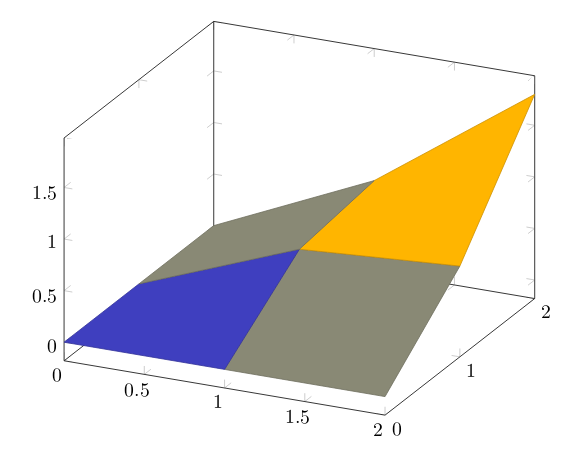
\includegraphics[width=8cm]{Imagenes/Pgfplot3d3}
    \captionof{chart}{Three dimensional graph.}
    \label{cha:chart1}
    \end{chart}
    
    \begin{figure}[h]
    \centering
    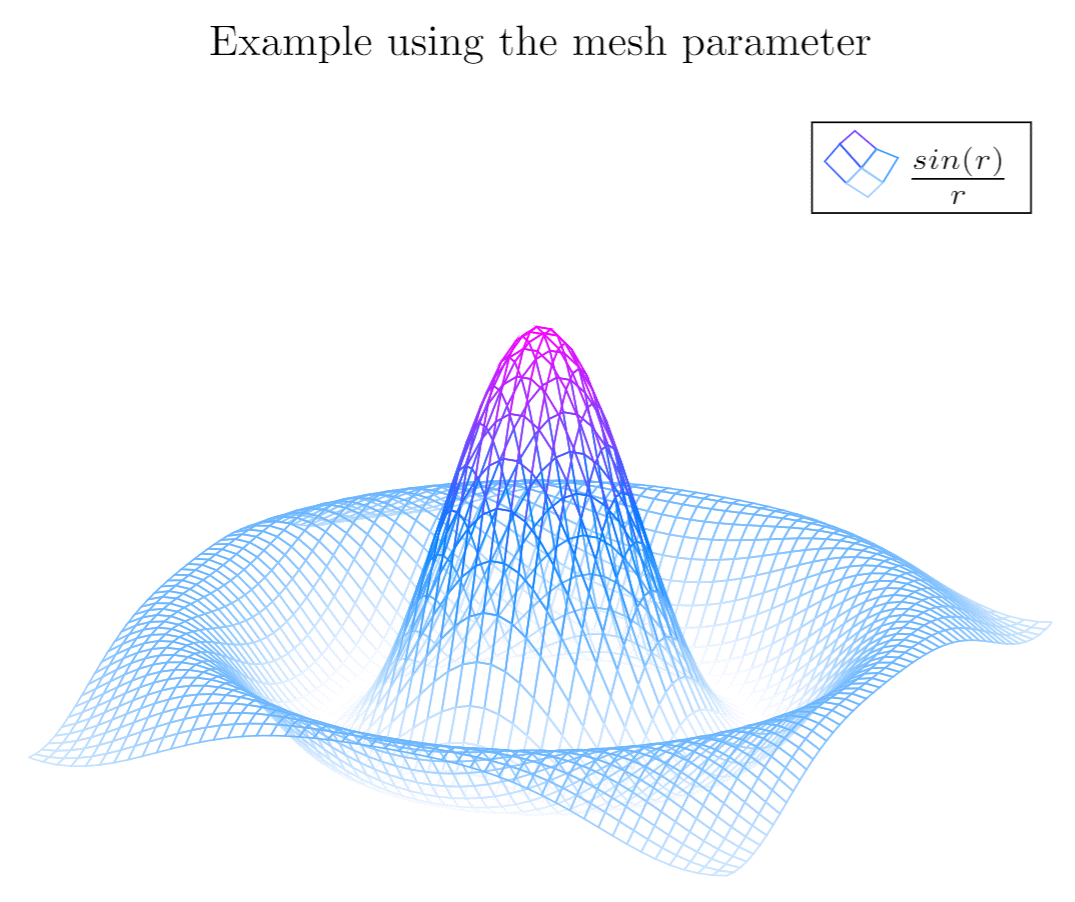
\includegraphics[width=0.5\textwidth]{Imagenes/pgfplots3dexample.png}
    \caption{Second 3D plot.}
    \label{fig:figure1}
    \end{figure}

    \begin{illustration}
        \caption{This is an example caption.}
        \label{ill:blah}  
        \begin{itemize}
          \item Possible illustration
        \end{itemize}
      \end{illustration}
%-------------------------------------------------------------------
\section*{\ProximoCapitulo}
%-------------------------------------------------------------------
\TocProximoCapitulo

...

% Variable local para emacs, para  que encuentre el fichero maestro de
% compilaci�n y funcionen mejor algunas teclas r�pidas de AucTeX
%%%
%%% Local Variables:
%%% mode: latex
%%% TeX-master: "../Tesis.tex"
%%% End:

%\include{...}
%\include{...}
%\include{...}
%\include{...}
%\include{...}

% Ap�ndices
\appendix
%---------------------------------------------------------------------
%
%                          Parte 3
%
%---------------------------------------------------------------------
%
% Parte3.tex
% Copyright 2009 Marco Antonio Gomez-Martin, Pedro Pablo Gomez-Martin
%
% This file belongs to the TeXiS manual, a LaTeX template for writting
% Thesis and other documents. The complete last TeXiS package can
% be obtained from http://gaia.fdi.ucm.es/projects/texis/
%
% Although the TeXiS template itself is distributed under the 
% conditions of the LaTeX Project Public License
% (http://www.latex-project.org/lppl.txt), the manual content
% uses the CC-BY-SA license that stays that you are free:
%
%    - to share & to copy, distribute and transmit the work
%    - to remix and to adapt the work
%
% under the following conditions:
%
%    - Attribution: you must attribute the work in the manner
%      specified by the author or licensor (but not in any way that
%      suggests that they endorse you or your use of the work).
%    - Share Alike: if you alter, transform, or build upon this
%      work, you may distribute the resulting work only under the
%      same, similar or a compatible license.
%
% The complete license is available in
% http://creativecommons.org/licenses/by-sa/3.0/legalcode
%
%---------------------------------------------------------------------

% Definici�n de la �ltima parte del manual, los ap�ndices

\partTitle{Ap�ndices}

\makepart

%---------------------------------------------------------------------
%
%                          Ap�ndice 1
%
%---------------------------------------------------------------------

\chapter{As� se hizo...}
\label{ap1:AsiSeHizo}

\begin{FraseCelebre}
\begin{Frase}
...
\end{Frase}
\begin{Fuente}
...
\end{Fuente}
\end{FraseCelebre}

\begin{resumen}
...
\end{resumen}

%-------------------------------------------------------------------
\section{Introducci�n}
%-------------------------------------------------------------------
\label{ap1:intro}

...

% Variable local para emacs, para  que encuentre el fichero maestro de
% compilaci�n y funcionen mejor algunas teclas r�pidas de AucTeX
%%%
%%% Local Variables:
%%% mode: latex
%%% TeX-master: "../Tesis.tex"
%%% End:

%\include{...}
%\include{...}
%\include{...}

\backmatter

%
% Bibliograf�a
%

%---------------------------------------------------------------------
%
%                      configBibliografia.tex
%
%---------------------------------------------------------------------
%
% bibliografia.tex
% Copyright 2009 Marco Antonio Gomez-Martin, Pedro Pablo Gomez-Martin
%
% This file belongs to the TeXiS manual, a LaTeX template for writting
% Thesis and other documents. The complete last TeXiS package can
% be obtained from http://gaia.fdi.ucm.es/projects/texis/
%
% Although the TeXiS template itself is distributed under the 
% conditions of the LaTeX Project Public License
% (http://www.latex-project.org/lppl.txt), the manual content
% uses the CC-BY-SA license that stays that you are free:
%
%    - to share & to copy, distribute and transmit the work
%    - to remix and to adapt the work
%
% under the following conditions:
%
%    - Attribution: you must attribute the work in the manner
%      specified by the author or licensor (but not in any way that
%      suggests that they endorse you or your use of the work).
%    - Share Alike: if you alter, transform, or build upon this
%      work, you may distribute the resulting work only under the
%      same, similar or a compatible license.
%
% The complete license is available in
% http://creativecommons.org/licenses/by-sa/3.0/legalcode
%
%---------------------------------------------------------------------
%
% Fichero  que  configura  los  par�metros  de  la  generaci�n  de  la
% bibliograf�a.  Existen dos  par�metros configurables:  los ficheros
% .bib que se utilizan y la frase c�lebre que aparece justo antes de la
% primera referencia.
%
%---------------------------------------------------------------------


%%%%%%%%%%%%%%%%%%%%%%%%%%%%%%%%%%%%%%%%%%%%%%%%%%%%%%%%%%%%%%%%%%%%%%
% Definici�n de los ficheros .bib utilizados:
% \setBibFiles{<lista ficheros sin extension, separados por comas>}
% Nota:
% Es IMPORTANTE que los ficheros est�n en la misma l�nea que
% el comando \setBibFiles. Si se desea utilizar varias l�neas,
% terminarlas con una apertura de comentario.
%%%%%%%%%%%%%%%%%%%%%%%%%%%%%%%%%%%%%%%%%%%%%%%%%%%%%%%%%%%%%%%%%%%%%%
\setBibFiles{%
nuestros,latex,otros%
}

%%%%%%%%%%%%%%%%%%%%%%%%%%%%%%%%%%%%%%%%%%%%%%%%%%%%%%%%%%%%%%%%%%%%%%
% Definici�n de la frase c�lebre para el cap�tulo de la
% bibliograf�a. Dentro normalmente se querr� hacer uso del entorno
% \begin{FraseCelebre}, que contendr� a su vez otros dos entornos,
% un \begin{Frase} y un \begin{Fuente}.
%
% Nota:
% Si no se quiere cita, se puede eliminar su definici�n (en la
% macro setCitaBibliografia{} ).
%%%%%%%%%%%%%%%%%%%%%%%%%%%%%%%%%%%%%%%%%%%%%%%%%%%%%%%%%%%%%%%%%%%%%%
\setCitaBibliografia{
\begin{FraseCelebre}
\begin{Frase}
  Y as�, del mucho leer y del poco dormir, se le sec� el celebro de
  manera que vino a perder el juicio.
\end{Frase}
\begin{Fuente}
  Miguel de Cervantes Saavedra
\end{Fuente}
\end{FraseCelebre}
}

%%
%% Creamos la bibliografia
%%
\makeBib

% Variable local para emacs, para  que encuentre el fichero maestro de
% compilaci�n y funcionen mejor algunas teclas r�pidas de AucTeX

%%%
%%% Local Variables:
%%% mode: latex
%%% TeX-master: "../Tesis.tex"
%%% End:


%
% �ndice de palabras
%

% sólo  la   generamos  si  está   declarada  \generaindice.  Consulta
% TeXiS.sty para m�s información.

% En realidad, el soporte para la generación de índices de palabras
% en TeXiS no está documentada en el manual, porque no ha sido usada
% "en producción". Por tanto, el fichero que genera el índice
% *no* se incluye aquí (está comentado). Consulta la documentación
% en TeXiS_pream.tex para más información.
\ifx\generaindice\undefined
\else
%%---------------------------------------------------------------------
%
%                        TeXiS_indice.tex
%
%---------------------------------------------------------------------
%
% TeXiS_indice.tex
% Copyright 2009 Marco Antonio Gomez-Martin, Pedro Pablo Gomez-Martin
%
% This file belongs to TeXiS, a LaTeX template for writting
% Thesis and other documents. The complete last TeXiS package can
% be obtained from http://gaia.fdi.ucm.es/projects/texis/
%
% This work may be distributed and/or modified under the
% conditions of the LaTeX Project Public License, either version 1.3
% of this license or (at your option) any later version.
% The latest version of this license is in
%   http://www.latex-project.org/lppl.txt
% and version 1.3 or later is part of all distributions of LaTeX
% version 2005/12/01 or later.
%
% This work has the LPPL maintenance status `maintained'.
% 
% The Current Maintainers of this work are Marco Antonio Gomez-Martin
% and Pedro Pablo Gomez-Martin
%
%---------------------------------------------------------------------
%
% Contiene  los  comandos  para  generar  el índice  de  palabras  del
% documento.
%
%---------------------------------------------------------------------
%
% NOTA IMPORTANTE: el  soporte en TeXiS para el  índice de palabras es
% embrionario, y  de hecho  ni siquiera se  describe en el  manual. Se
% proporciona  una infraestructura  básica (sin  terminar)  para ello,
% pero  no ha  sido usada  "en producción".  De hecho,  a pesar  de la
% existencia de  este fichero, *no* se incluye  en Tesis.tex. Consulta
% la documentación en TeXiS_pream.tex para m�s información.
%
%---------------------------------------------------------------------


% Si se  va a generar  la tabla de  contenidos (el índice  habitual) y
% tambi�n vamos a  generar el índice de palabras  (ambas decisiones se
% toman en  función de  la definición  o no de  un par  de constantes,
% puedes consultar modo.tex para m�s información), entonces metemos en
% la tabla de contenidos una  entrada para marcar la página donde est�
% el índice de palabras.

\ifx\generatoc\undefined
\else
   \addcontentsline{toc}{chapter}{\indexname}
\fi

% Generamos el índice
\printindex

% Variable local para emacs, para  que encuentre el fichero maestro de
% compilación y funcionen mejor algunas teclas r�pidas de AucTeX

%%%
%%% Local Variables:
%%% mode: latex
%%% TeX-master: "./tesis.tex"
%%% End:

\fi

%
% Lista de acr�nimos
%

% sólo  lo  generamos  si  está declarada  \generaacronimos.  Consulta
% TeXiS.sty para m�s información.


\ifx\generaacronimos\undefined
\else
%---------------------------------------------------------------------
%
%                        TeXiS_acron.tex
%
%---------------------------------------------------------------------
%
% TeXiS_acron.tex
% Copyright 2009 Marco Antonio Gomez-Martin, Pedro Pablo Gomez-Martin
%
% This file belongs to TeXiS, a LaTeX template for writting
% Thesis and other documents. The complete last TeXiS package can
% be obtained from http://gaia.fdi.ucm.es/projects/texis/
%
% This work may be distributed and/or modified under the
% conditions of the LaTeX Project Public License, either version 1.3
% of this license or (at your option) any later version.
% The latest version of this license is in
%   http://www.latex-project.org/lppl.txt
% and version 1.3 or later is part of all distributions of LaTeX
% version 2005/12/01 or later.
%
% This work has the LPPL maintenance status `maintained'.
% 
% The Current Maintainers of this work are Marco Antonio Gomez-Martin
% and Pedro Pablo Gomez-Martin
%
%---------------------------------------------------------------------
%
% Contiene  los  comandos  para  generar  el listado de acr�nimos
% documento.
%
%---------------------------------------------------------------------
%
% NOTA IMPORTANTE:  para que la  generaci�n de acr�nimos  funcione, al
% menos  debe  existir  un  acr�nimo   en  el  documento.  Si  no,  la
% compilaci�n  del   fichero  LaTeX  falla  con   un  error  "extra�o"
% (indicando  que  quiz�  falte  un \item).   Consulta  el  comentario
% referente al paquete glosstex en TeXiS_pream.tex.
%
%---------------------------------------------------------------------


% Redefinimos a espa�ol  el t�tulo de la lista  de acr�nimos (Babel no
% lo hace por nosotros esta vez)

\def\listacronymname{Lista de acr\'onimos}

% Para el glosario:
% \def\glosarryname{Glosario}

% Si se  va a generar  la tabla de  contenidos (el �ndice  habitual) y
% tambi�n vamos a  generar la lista de acr�nimos  (ambas decisiones se
% toman en  funci�n de  la definici�n  o no de  un par  de constantes,
% puedes consultar config.tex  para m�s informaci�n), entonces metemos
% en la  tabla de contenidos una  entrada para marcar  la p�gina donde
% est� el �ndice de palabras.

\ifx\generatoc\undefined
\else
   \addcontentsline{toc}{chapter}{\listacronymname}
\fi


% Generamos la lista de acr�nimos (en realidad el �ndice asociado a la
% lista "acr" de GlossTeX)

\printglosstex(acr)

% Variable local para emacs, para  que encuentre el fichero maestro de
% compilaci�n y funcionen mejor algunas teclas r�pidas de AucTeX

%%%
%%% Local Variables:
%%% mode: latex
%%% TeX-master: "../Tesis.tex"
%%% End:

\fi

%
% Final
%
%---------------------------------------------------------------------
%
%                      fin.tex
%
%---------------------------------------------------------------------
%
% fin.tex
% Copyright 2009 Marco Antonio Gomez-Martin, Pedro Pablo Gomez-Martin
%
% This file belongs to the TeXiS manual, a LaTeX template for writting
% Thesis and other documents. The complete last TeXiS package can
% be obtained from http://gaia.fdi.ucm.es/projects/texis/
%
% Although the TeXiS template itself is distributed under the 
% conditions of the LaTeX Project Public License
% (http://www.latex-project.org/lppl.txt), the manual content
% uses the CC-BY-SA license that stays that you are free:
%
%    - to share & to copy, distribute and transmit the work
%    - to remix and to adapt the work
%
% under the following conditions:
%
%    - Attribution: you must attribute the work in the manner
%      specified by the author or licensor (but not in any way that
%      suggests that they endorse you or your use of the work).
%    - Share Alike: if you alter, transform, or build upon this
%      work, you may distribute the resulting work only under the
%      same, similar or a compatible license.
%
% The complete license is available in
% http://creativecommons.org/licenses/by-sa/3.0/legalcode
%
%---------------------------------------------------------------------
%
% Contiene la �ltima p�gina
%
%---------------------------------------------------------------------


% Ponemos el marcador en el PDF al nivel adecuado, dependiendo
% de su hubo partes en el documento o no (si las hay, queremos
% que aparezca "al mismo nivel" que las partes.
\ifpdf
\ifx\tienePartesTeXiS\undefined
   \pdfbookmark[0]{Fin}{fin}
\else
   \pdfbookmark[-1]{Fin}{fin}
\fi
\fi

\thispagestyle{empty}\mbox{}

\vspace*{4cm}

\small

\hfill \emph{--�Qu� te parece desto, Sancho? -- Dijo Don Quijote --}

\hfill \emph{Bien podr�n los encantadores quitarme la ventura,}

\hfill \emph{pero el esfuerzo y el �nimo, ser� imposible.}

\hfill 

\hfill \emph{Segunda parte del Ingenioso Caballero} 

\hfill \emph{Don Quijote de la Mancha}

\hfill \emph{Miguel de Cervantes}

\vfill%space*{4cm}

\hfill \emph{--Buena est� -- dijo Sancho --; f�rmela vuestra merced.}

\hfill \emph{--No es menester firmarla -- dijo Don Quijote--,}

\hfill \emph{sino solamente poner mi r�brica.}

\hfill 

\hfill \emph{Primera parte del Ingenioso Caballero} 

\hfill \emph{Don Quijote de la Mancha}

\hfill \emph{Miguel de Cervantes}


\newpage
\thispagestyle{empty}\mbox{}

\newpage

% Variable local para emacs, para  que encuentre el fichero maestro de
% compilaci�n y funcionen mejor algunas teclas r�pidas de AucTeX

%%%
%%% Local Variables:
%%% mode: latex
%%% TeX-master: "../Tesis.tex"
%%% End:


\end{document}
